
\section{Validation Metrics} 
\label{sec:validation-metrics}

There are various methods and algorithms available to evaluate the similarity between two or more seismograms, both through direct quantitative comparisons or indirect statistical analysis \citep[e.g.,][]{Anderson_2004_Proc, Kristekova_2006_BSSA, Kristekova_2009_GJI, Olsen_2010_SRL, Burks_BSSA_2014, Rezaeian_2015_BSSA}. In earthquake ground motion simulation, they are primarily used for verification with respect to benchmark or analytical solutions, and for validation with respect to data (i.e., ground motion records). Here, we focus on the list of metrics proposed by \citet{Anderson_2004_Proc}, with an additional metric for duration, as suggested by others \citep{Olsen_2010_SRL, Maufroy_2015_BSSA} and as implemented in \citet{Taborda_2013_BSSA}.


\begin{table}[t]
\caption{Validation Metrics}
\centering
\small
\begin{tabular}{ll}
	\hline
	\multicolumn{1}{c}{Code}          & 
	\multicolumn{1}{c}{Metric}        \\
	\hline
	C1   & Arias Intensity Integral   \\
	C2   & Energy Integral            \\
	C3   & Arias Intensity		      \\
	C4   & Total Energy               \\
	C5   & Peak Acceleration          \\
	C6   & Peak Velocity              \\
	C7   & Peak Displacement          \\
	C8   & Response Spectrum          \\
	C9   & Fourier Amplitude Spectrum \\
	C10  & Cross Correlation          \\
	C11  & Strong Phase Duration      \\
	\hline
\end{tabular}
\label{tab:metrics}
\end{table}


These metrics are listed in Table \ref{tab:metrics}. Following \citet{Anderson_2004_Proc}, when applied to a pair of signals, each one of these metrics yields a GOF score ranging from 0 to 10, where a value of 10 corresponds to two signals having identical characteristics. This scoring scale varies according to the following exponential function:
% 
\begin{equation}
\label{eq:gof-function}
	S \left( p_1, p_2 \right) = 10 \exp{ \left[ - \left( \frac{p_1 - p_2}{ \min\left( p_1, p_2 \right) } \right)^2 \right] }
	\, ,
\end{equation}
% 
\noindent
where $S$ is the GOF score that results from comparing values $p_1$ and $p_2$ from signals 1 and 2, respectively, for each one of the different metrics in Table \ref{tab:metrics}. \citeauthor{Anderson_2004_Proc} also provided guidelines for the process to be applied to the original signals as well as to those resulting from a sequential set of band-pass filters covering the whole frequency range of interest. In his method, this frequency-domain decomposition should have pass bands defined following a logarithmic distribution in order to give more weight to the low-frequencies, and the GOF scores of all sub-bands and the broadband be averaged into a single GOF final score.

\begin{figure*}
    \centering
    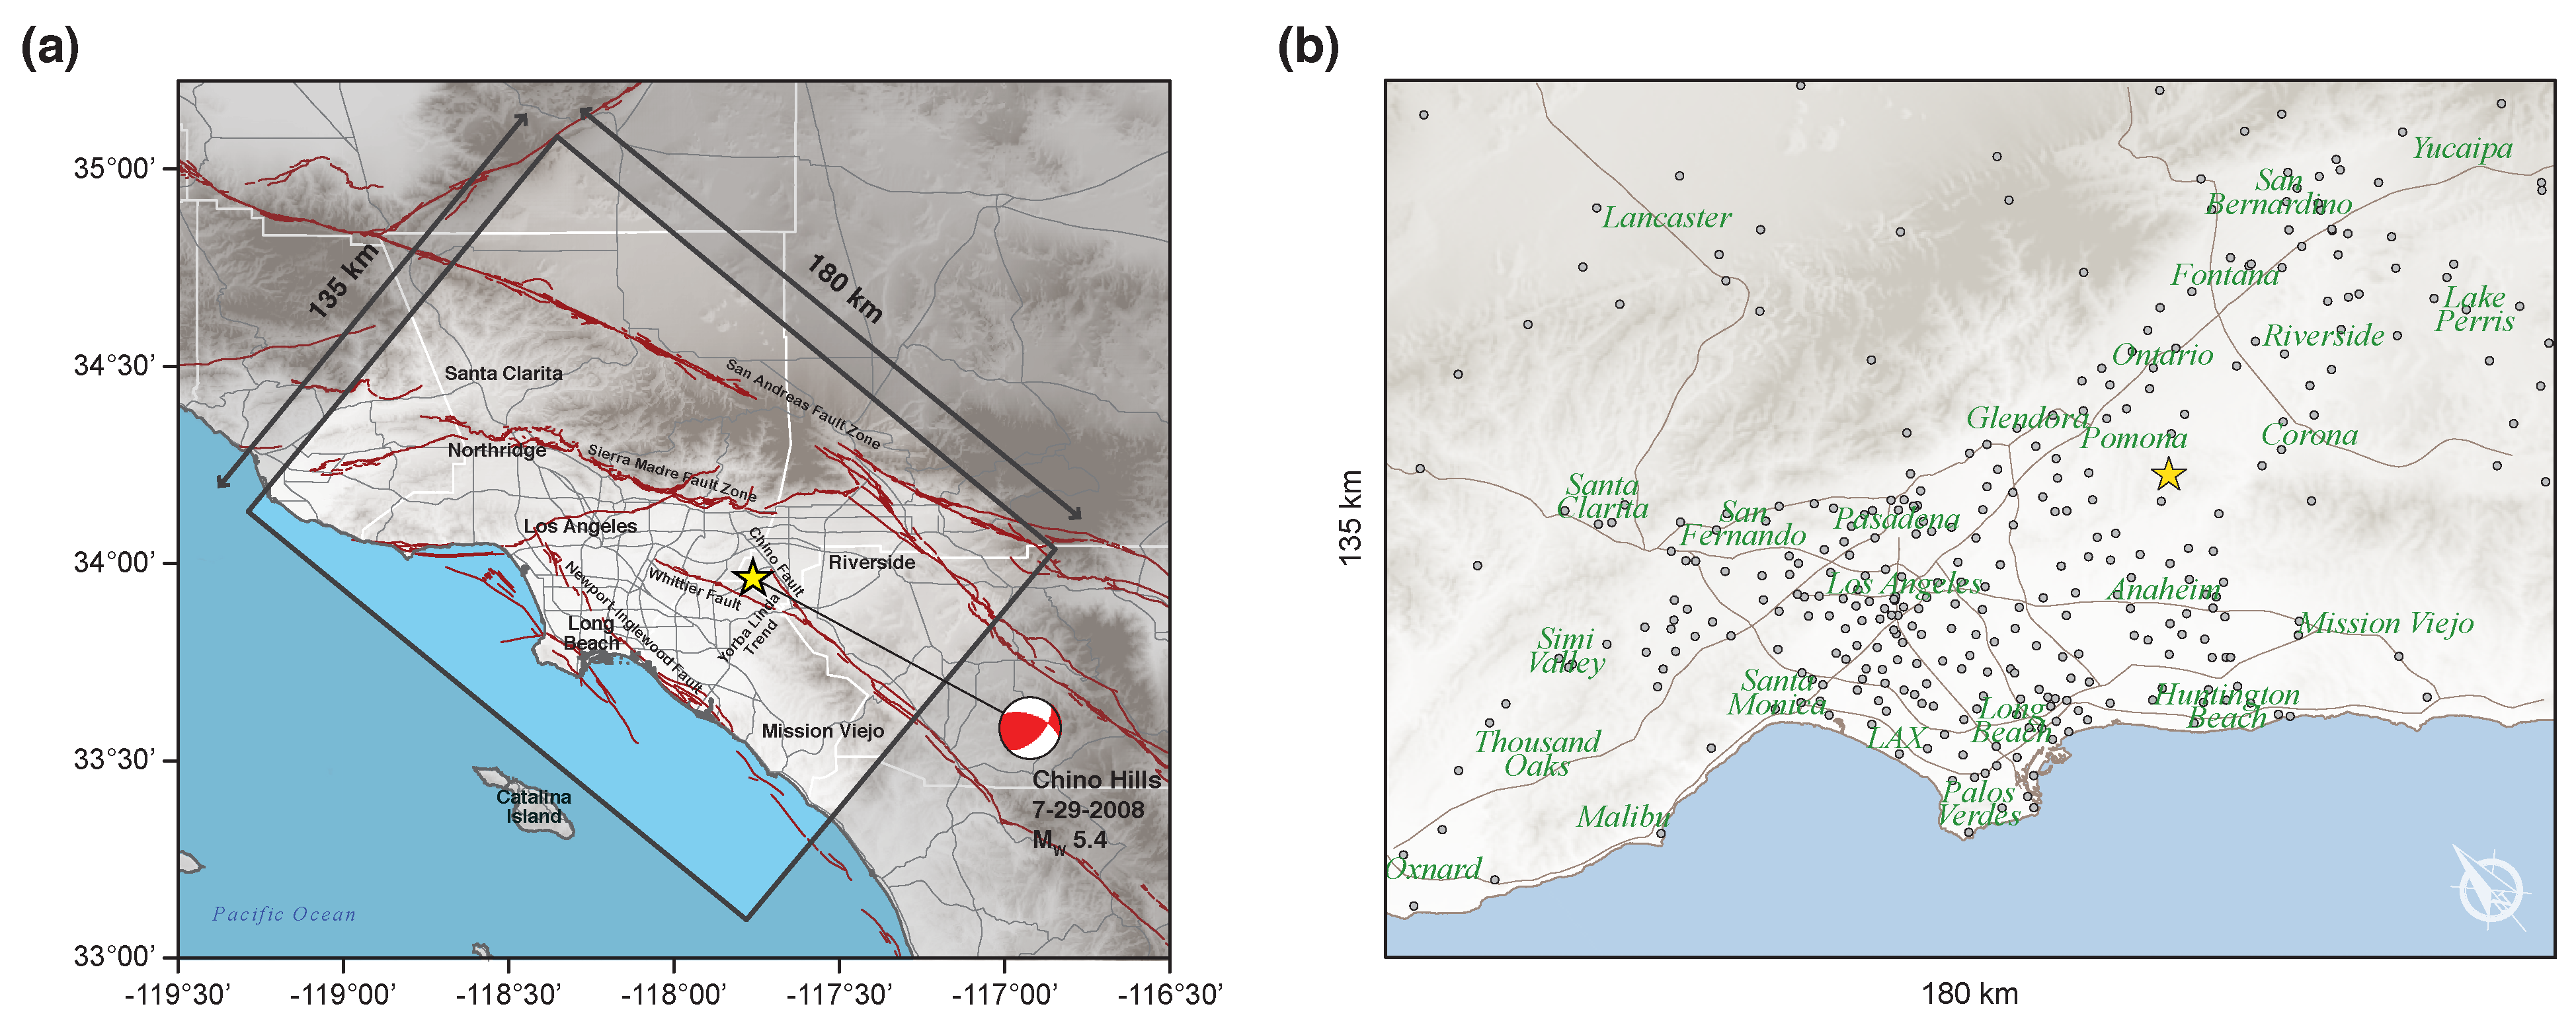
\includegraphics[width=\textwidth]{figures/pdf/figure-01}
    \caption{\textbf{(a)} Region of interest used by \citet{Taborda_2014_BSSA} for the simulations of the 2008 $M_W ~ 5.4$ Chino Hills earthquake, including the epicenter, focal mechanism, and major quaternary faults. In the background, the main roads and topography are shown for visual reference. \textbf{(b)} Distribution of the 336 stations (gray dots) used by \citet{Taborda_2014_BSSA} for the validation analysis of their simulations within the modeling domain shown in part (a). Roads, city names, and the hillshade topography are also shown here in the background for reference. The color version of this figure is available only in the electronic edition.}
    \label{fig:chino-hills}
\end{figure*}

\citet{Anderson_2004_Proc} calibrated the results of GOF scores comparing horizontal components of recorded seismograms and other simulations using the first ten metrics (C1 through C10) in Table \ref{tab:metrics}. He concluded that for a typical distribution of the scores, the GOF could be categorized into four groups: poor (for scores from 0 to 4), fair (4 to 6), good (6 to 8), and excellent (for scores from 8 to 10). While this categorization was arguably subjective, over the years it has become common practice and has been adopted or matched by alternative validation methods \citep[e.g.,][]{Kristekova_2009_GJI, Olsen_2010_SRL}, making the method itself a reference baseline for various validation studies \citep[e.g.,][]{Chaljub_2010_BSSA, Bielak_2010_GJI, Guidotti_2011_SRL, Maufroy_2015_BSSA}.

Here, we focus our analysis on the eleven metrics included in Table \ref{tab:metrics}, and investigate the relationships that exist between them in order to prioritize a reduced number of metrics that can help predict the outcome category one would use to label the results of a given simulation.
